\chapter{Regresión Lineal}

\section{Algoritmo de la Pseudo-inversa}
El algoritmo de la Pseudo-inversa o mínimos cuadrados ordinarios consiste
en minimizar el error cuadrático entre la estimación $h(x) = w^T x$ y
el vector objetivo $y$

\begin{equation}
E_{in}(h) = \frac{1}{N} \sum_{n=1}^N (h(x_n) - y_n)^2 = \frac{1}{N} \Vert Xw - y\Vert^2
\end{equation}

Basta encontrar $w$ que anule $\nabla E_{in}(w)$. Esto se verifica cuando
$w_{lin} = X^\dagger y$ \cite{LFD}. Donde $X^\dagger = (X^T X)^{-1} X^T$ es la
\textbf{matriz pseudo-inversa} de $X$

Como el cálculo de la inversa $(X^T X)^{-1}$ puede ser costoso, aplicamos
previamente la descomposición en valores singulares a $X$. Es decir, escribimos
$X = U D V^T $ con $U \in \mathbb{R}^{N \times N}$, $V \in \mathbb{R}^{(d+1) \times (d+1)}$
matrices ortogonales y $D \in \mathbb{R}^{N \times (d+1)}$ matriz diagonal rectangular.
Entonces $X^T X = V D^T D V^T$ y la pseudo-inversa se calculará como sigue:

\begin{equation}
\begin{aligned}
X^\dagger = (X^T X)^{-1} X^T = (V D^T D V^T)^{-1} V D^T U^T = \\
= V (D^T D)^{-1} V^T V D^T U^T= V (D^T D)^{-1} D^T U^T = V D^\dagger U^T
\end{aligned}
\end{equation}


\section{Gradiente Descendente Estocástico}

El algoritmo de gradiente descendente estocástico (SGD) es una versión secuencial
del algoritmo de gradiente descendente descrito en el primer capítulo.
En esta versión, usamos sólo una parte de la muestra para calcular el
gradiente. Para ello, dividimos la muestra aleatoriamente en
\textbf{mini-batches}. Recorreremos esta secuencia de lotes, actualizando los
pesos en cada mini-batch de manera que sólo uno participa en cada actualización.

Formalmente, para cada mini-batch $B_i$ 

\begin{equation*}
  \frac{\partial E_{in}(w)}{\partial w_j} = \frac{2}{M} \sum_{n \in B_i} x_{nj} (h(x_n) - y_n)
\end{equation*}

\section{Ejercicio 1}

Este ejercicio ajusta modelos de regresión a vectores de características
extraídos a partir de imágenes de dígitos manuscritos. En particular, se
extraen dos características concretas que miden el valor medio del nivel de
gris y la simetría del dígito respecto de su eje vertical. Solo se
seleccionaran para este ejercicio las imágenes de los números 1 y 5.

\textbf{Estimar un modelo de regresión lineal}, a partir de los datos proporcionados
por los vectores de características dados, usando tanto el algoritmo de la
pseudo-inversa como el gradiente descendente estocástico (SGD). Las etiquetas
serán {-1,1}, una por cada vector de cada uno de los números. Pintar las
soluciones obtenidas junto con los datos usados en el ajuste. \textbf{Valorar la
bondad del resultado usando $E_{in}$ y $E_{out}$} (para $E_{out}$ calcular las
predicciones usando los datos del fichero de test).

\hfill \break

En el caso de la pseudo-inversa, se ha implementado usando la descomposición en
valores singulares anteriormente descrita en \mintinline{python}{def pseudoinverse(x):}
y se ha aplicado al problema de regresión con cierto vector objetivo $y$ en 
\mintinline{python}{def regresion_pinv(x, y)}.

En cuanto al algoritmo de gradiente descendente estocástico (SGD), se ha implementado
en su versión \textit{mini-batch} de forma general mediante una condición genérica de
parada, como se hizo con el no estocástico. Esta se ha particularizado para el caso 
de un batch de tamaño $32$ y una condición de parada por máximo de iteraciones en 

\begin{minted}{python}
def sgd_maxIter(x, y, lr, max_iters, epsilon=None, 
                batch_size=32, hist=False):
\end{minted}

También existe otra versión (\mintinline{python}{sgd_maxIter_error()}) con
condición de parada mixta por máximo de iteraciones o cota de error.

Tras cierta experimentación con los parámetros, se ha decidido exponer la comparación entre SGD con
un $500$ iteraciones, SGD con $20000$ iteraciones y el algoritmo de la
pseudoinversa. En particular, se ha escogido una tasa de aprendizaje 
$\eta = 0.01$ por la estabilidad proporcionada.

\begin{figure}[H]
\centering
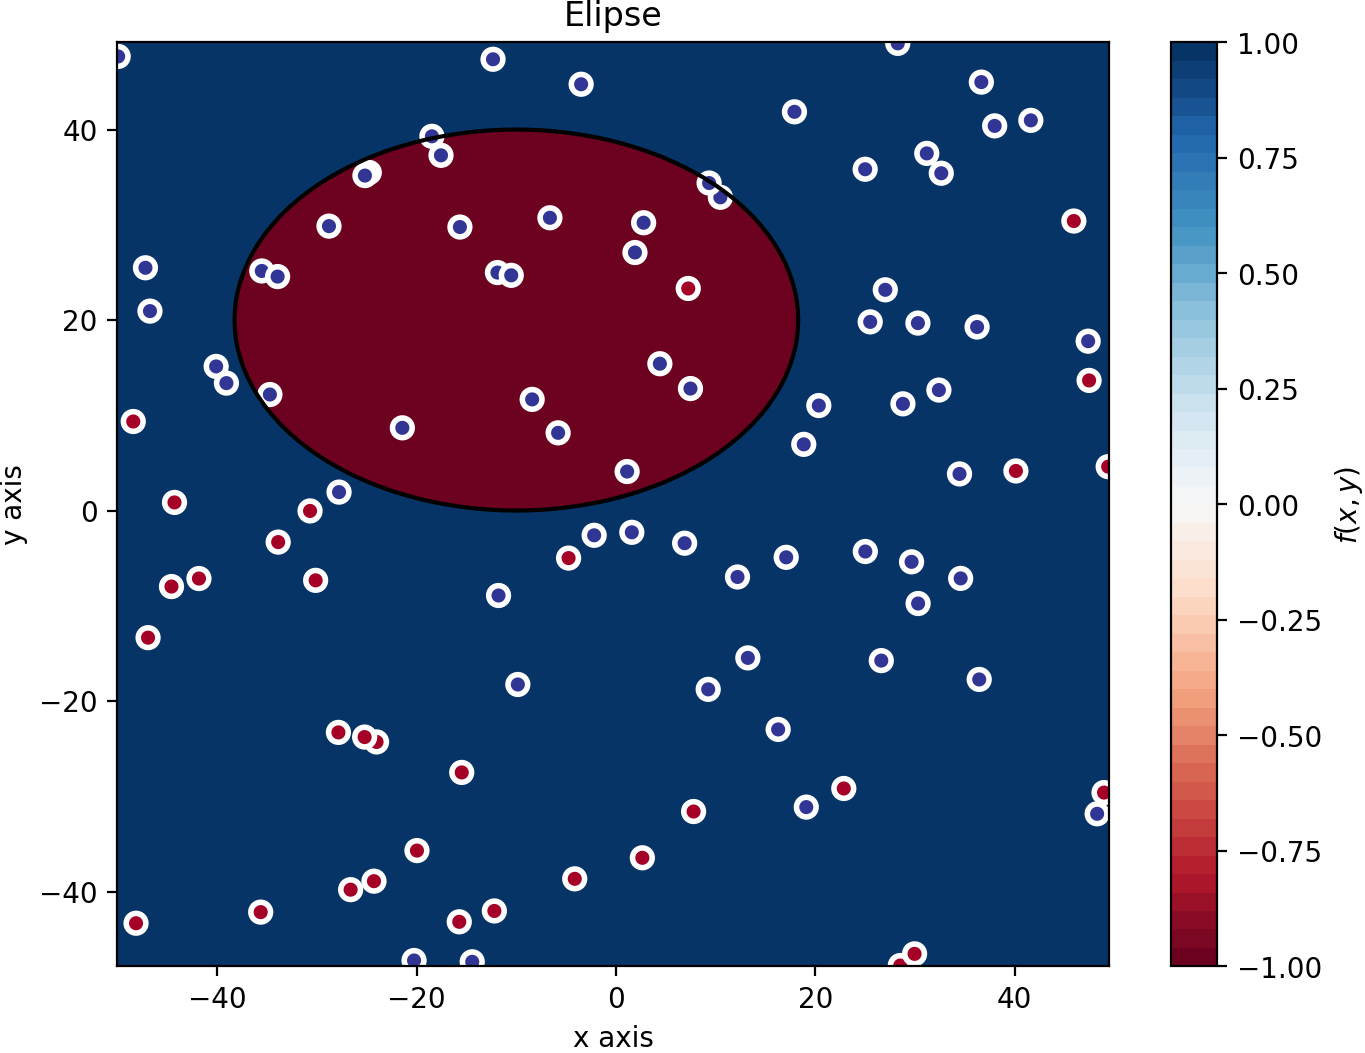
\includegraphics[scale=0.6]{Figure_6.png}
\caption{Descenso del gradiente sobre f con $\eta=0.01$}
\end{figure}

\begin{table}[!ht]
    \centering
    \begin{tabular}{llll} 
    \toprule
        Algoritmo & Iteraciones & $E_{in}$ & $E_{out}$ \\ \midrule
        SGD (32)  & 500 & 0.083469 & 0.132706 \\ 
        SGD (32) & 20000 & 0.080445 & 0.135549 \\ 
        Pseudoinversa  & ---- &  0.079187 & 0.130954 \\ \bottomrule
    \end{tabular}
\end{table}

Se observa que $E_{in}$ producido por la pseudoinversa es menor que el del
Gradiente Descendente Estocástico. Esto se debe a que el algoritmo de la
pseudoinversa se basa en la minimización de este error. Ahora bien, a partir
cierto tamaño de datos, este algoritmo se puede volver costoso por las operaciones
matriciales involucradas (si bien reducimos esta complejidad mediante la descomposición
en valores singulares). Además, el componente aleatorio de SGD permite escapar de mínimos
locales al contrario del algoritmo normal tratado en el capítulo 1.

En cuanto a las $E_{out}$ originados por las predicciones en test, vemos que son
mayores que los $E_{in}$. Esto sucede porque el algoritmo no se adapta a los datos
de test igual que a los datos con los que ha sido entrenado.

Finalmente, podemos notar a partir de la gráfica junto con experimentaciones con mayores
valores de iteraciones que el algoritmo de gradiente descendente estocástico
genera una recta de regresión que se acerca a la producida por el algoritmo de
la pseudoinversa conforme se aumentamos el número de iteraciones.


\section{Ejercicio 2}

En este apartado exploramos cómo se transforman los errores $E_{in}$ y $E_{out}$
cuando aumentamos la complejidad del modelo lineal usado. Ahora hacemos uso de
la función \mintinline{python}{simula_unif(N, 2, size)} que nos devuelve $N$
coordenadas 2D de puntos uniformemente muestreados dentro del cuadrado definido
por  $[−size,size] \times [−size, size]$. Se debe realizar el siguiente experimento:

\subsection{Generar muestra de entrenamiento}

\textbf{Generar una muestra de entrenamiento de $N = 1000$ puntos en el cuadrado
$\chi = [−1, 1] \times [−1, 1].$ Pintar el mapa de puntos 2D.}

\begin{figure}[H]
\centering
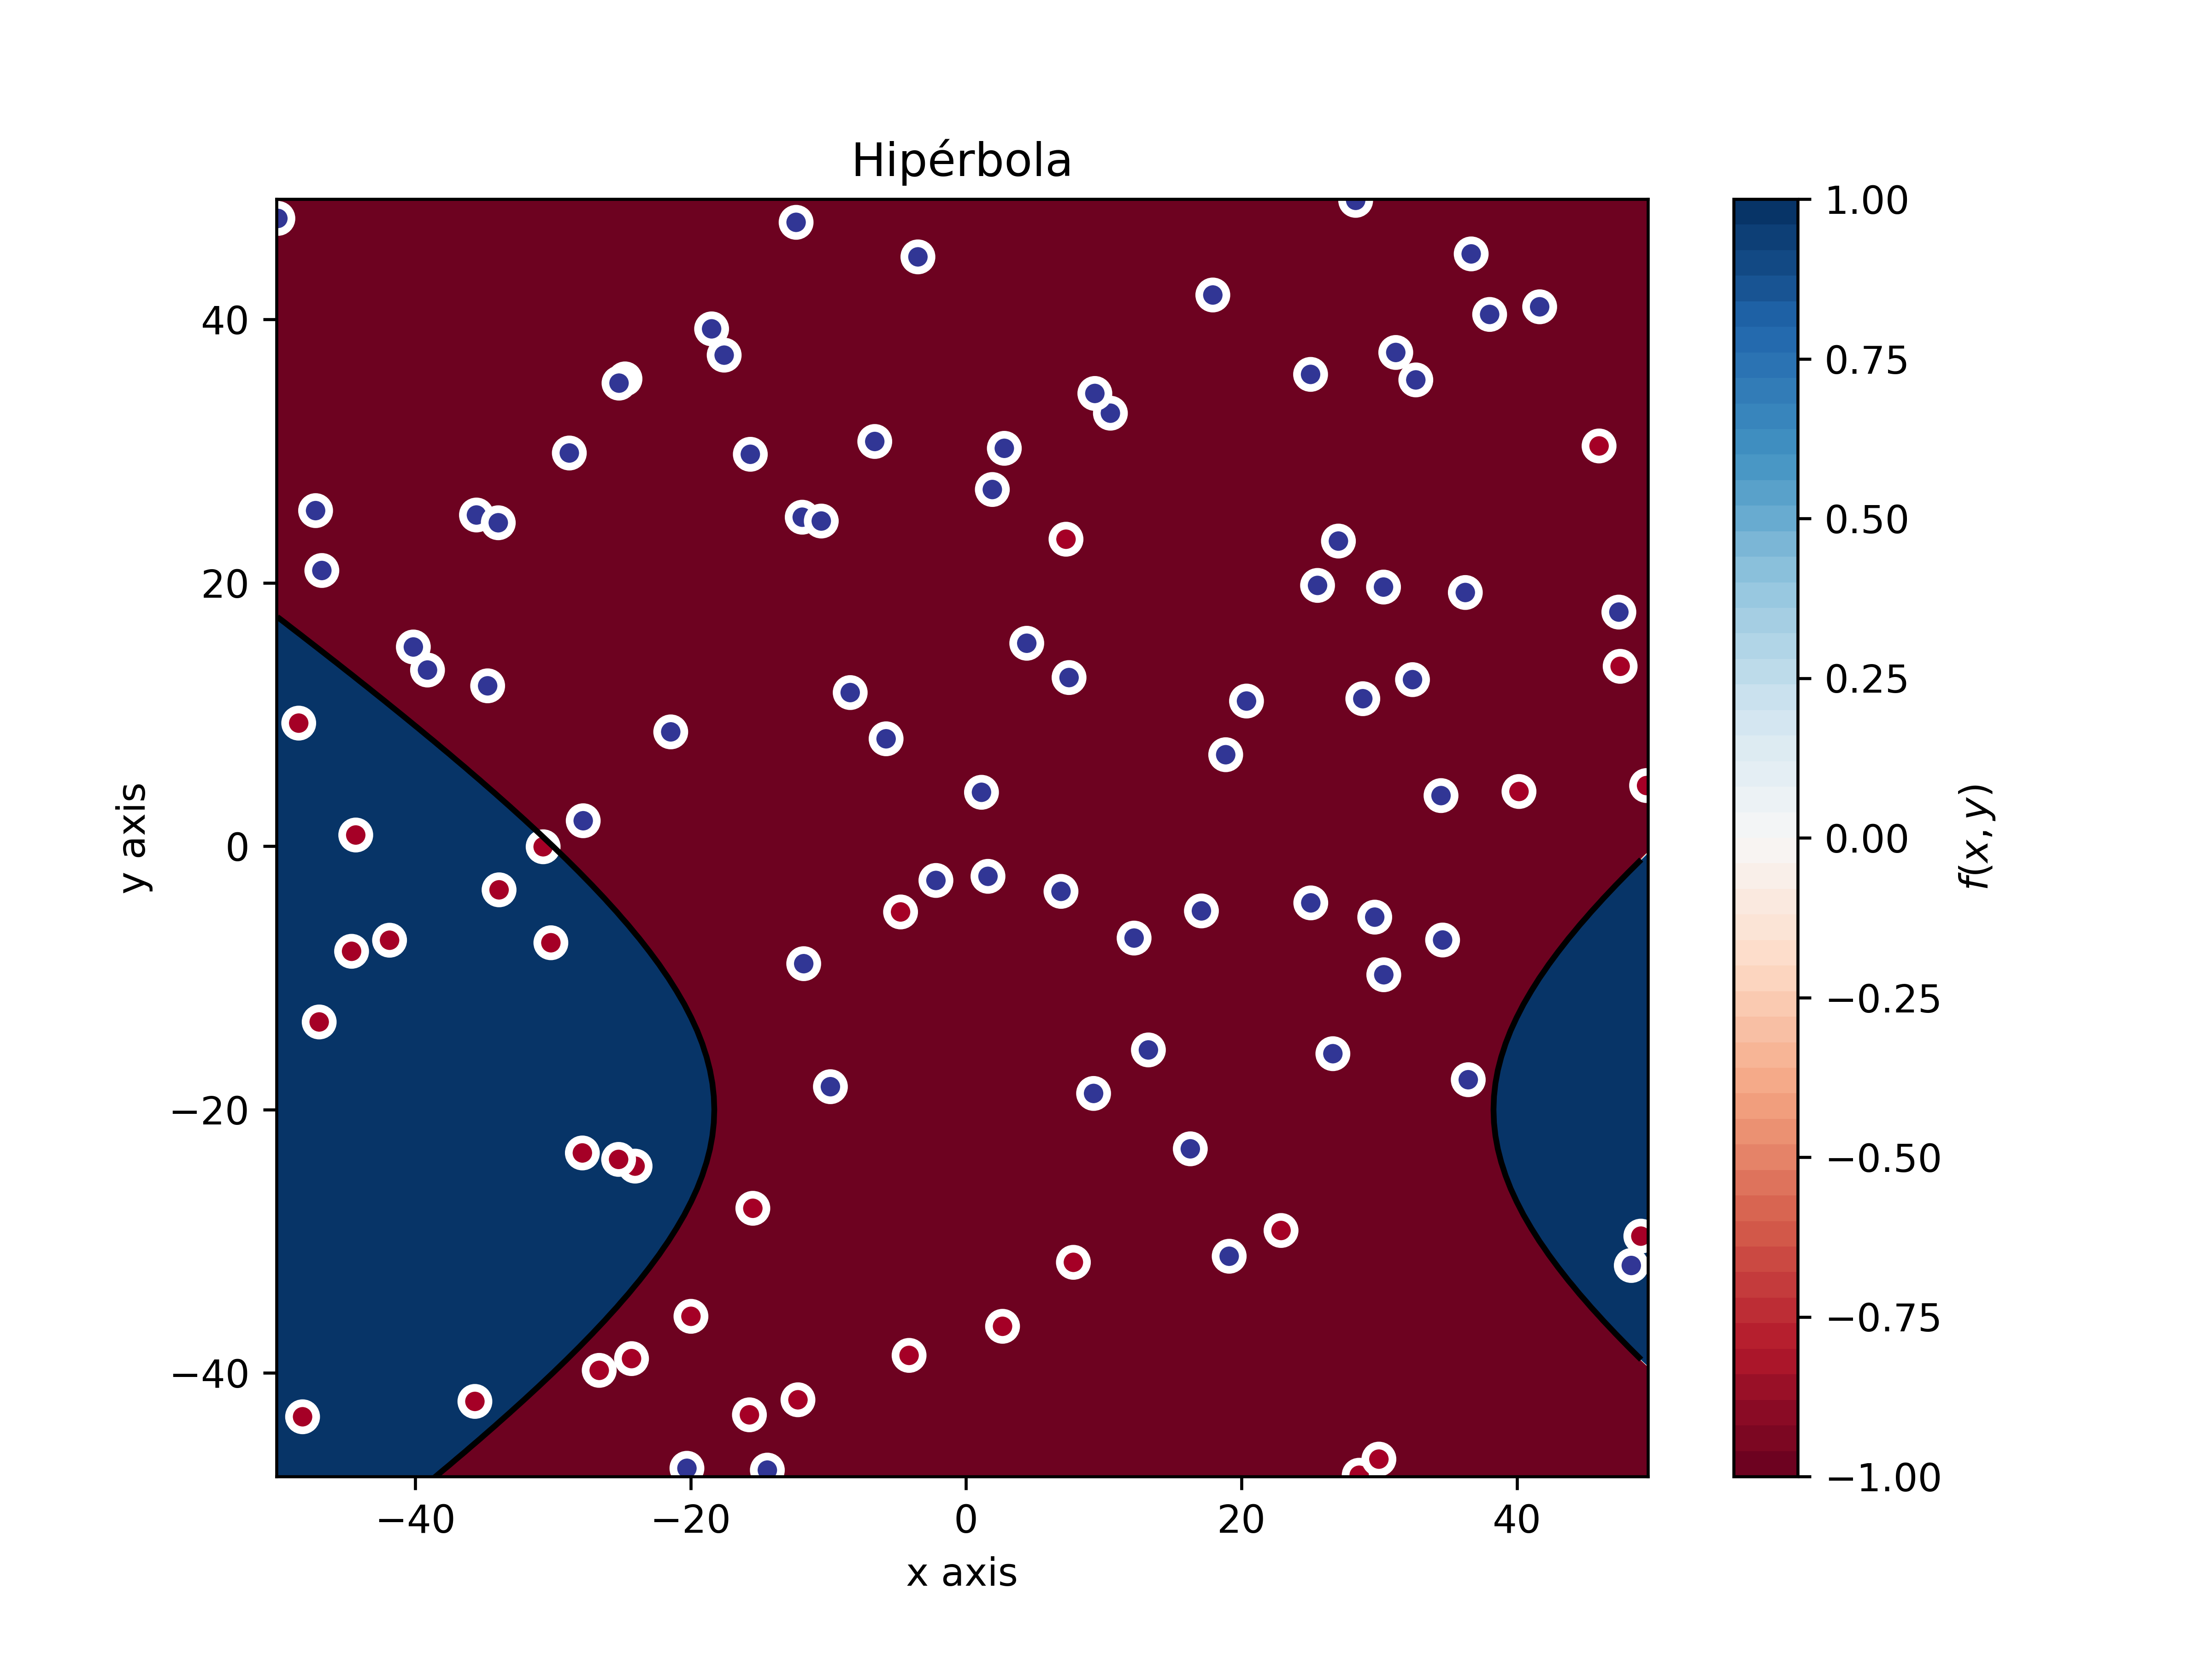
\includegraphics[scale=0.6]{Figure_7.png}
\caption{Muestra aleatoria uniforme con $N = 1000$ en $\chi=[-1, 1] \times [-1, 1]$}
\end{figure}


\subsection{Etiquetado de la muestra}

Consideremos la función $f(x_1, x_2) = sign\left( (x_1 − 0,2)^2 + x_2^2 − 0,6 \right)$ 
que usaremos para asignar una etiqueta a cada punto de la muestra anterior.
Introducimos ruido sobre las etiquetas cambiando el signo de un 10\%
de las mismas elegido aleatoriamente. \textbf{Pintar el mapa de etiquetas obtenido.}

\begin{figure}[H]
\centering
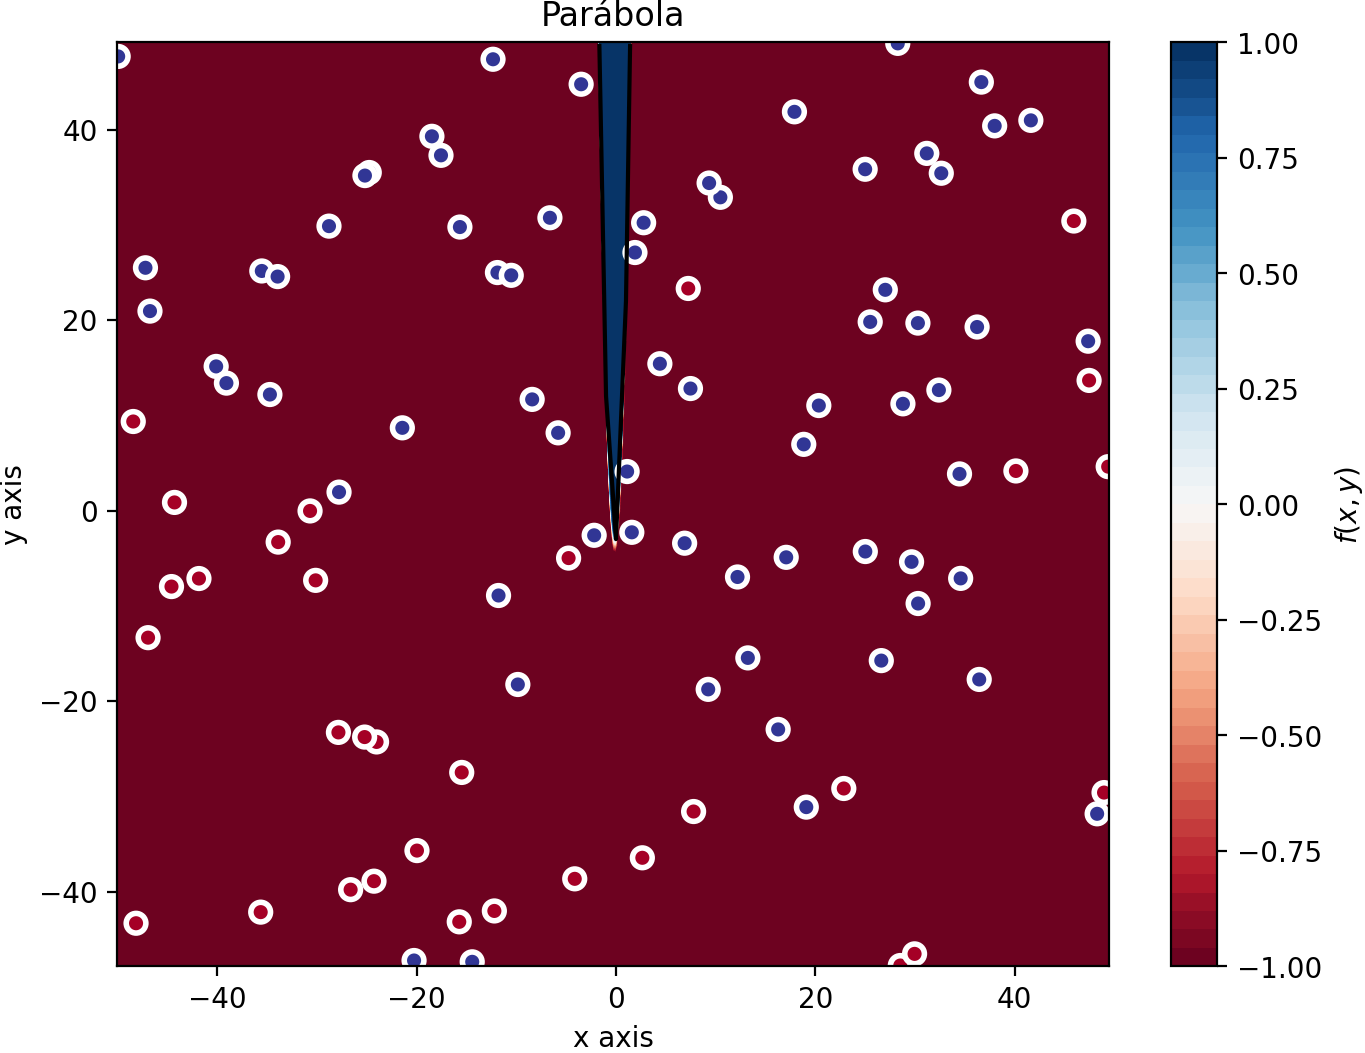
\includegraphics[scale=0.6]{Figure_8.png}
\caption{Etiquetado de la muestra según $f$ con ruido de $10\%$}
\end{figure}

Una vez generado el vector de etiquetas $y$ aplicando $f$ a la muestra, se ha añadido 
el ruido con \mintinline{python}{y[noise] = -y[noise]} siendo \mintinline{python}{noise}
un vector aleatorio uniforme de $0.1 \cdot N$ índices entre $0$ y $N$. 


\subsection{Modelo de regresión Lineal.}

Usando como vector de características $(1, x_1, x_2)$, ajustar un modelo de
regresion lineal al conjunto de datos generado y estimar los pesos w. 
\textbf{Estimar el error de ajuste $E_{in}$ usando SGD.}

Usando SGD con $\eta = 0.01$ y $200$ iteraciones, se ha obtenido:

\begin{itemize}
\item $E_{in} = 0.9293368608301051$
\item $w = [0.02527404, -0.35022946, -0.01136838]$
\end{itemize}

\begin{figure}[H]
\centering
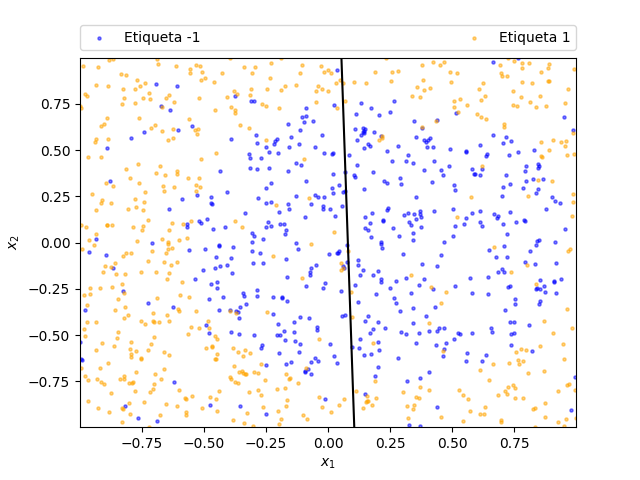
\includegraphics[scale=0.6]{Figure_9.png}
\caption{Modelo de regresión lineal a la muestra generada}
\end{figure}
  
En efecto, el error de ajuste es altísimo debido a que los valores se han
generado aleatoriamente con distribución uniforme y no se acercan a ningún
modelo lineal.

\subsection{Repetir experimento $1000$ veces}

\textbf{Ejecutar todo el experimento definido en los apartado anteriores 1000
veces (generamos 1000 muestras diferentes) y}

\begin{itemize}
  \item \textbf{Calcular el valor medio de los errores $E_{in}$ de las $1000$ muestras.}
  \item \textbf{Generar $1000$ puntos nuevos por cada iteración y calcular con ellos el
  valor de $E_{out}$ en dicha iteración.}
  \item \textbf{Calcular el valor medio de $E_{out}$ en todaslas iteraciones.}
\end{itemize}

Se ha decidido ejecutar por cada repetición, SGD con $200$ iteraciones para
obtener un resultado en no más de $10$ segundos. Los promedios de $E_{in}$ y
$E_{out}$ son respectivamente:

\begin{itemize}
  \item $E_{in}$ promedio: 0.9325394003097736
  \item $E_{out}$ promedio: 0.9357118616492284 
\end{itemize}


\textbf{Valore qué tan bueno considera que es el ajuste con este modelo lineal a la vista de los
valores medios obtenidos de $E_{in}$ y $E_{out}$.}

En efecto, los erores de ajuste obtenidos en promedio para $1000$ iteraciones del
experimento anterior no han producido una mejora significativa. Es claro de las figuras
obtenidas anteriormente, que un modelo lineal no separa etiquetas acumuladas en
circunferencia.

\section{Repetición del experimento con características no lineales}

\textbf{Repetir el mismo experimento anterior pero usando características no
lineales. Ahora usaremos el siguiente vector de características:}

$$
\phi_2(x) = (1, x_1, x_2, x_1 x_2, x_1^2, x_2^2)
$$

\textbf{Ajustar el nuevo modelo de regresión lineal y calcular el nuevo vector de pesos $\hat{w}$.
Calcular los errores promedio de $E_{in}$ y $E_{out}$.}

\hfill \break

Para la implementación, se ha decidido modificar la función \\
\mintinline{python}{generar_muestra_2D_uniforme(N, no_lineal)}
donde el parámetro \mintinline{python}{no_lineal} es un booleano
que indica si agregar las nuevas columnas.

Los errores promedio obtenidos en este caso, han sido los siguientes:

\begin{itemize}
\item $E_{in}$ promedio: $0.7736520275418629$
\item $E_{out}$ promedio: $0.7785544126191773$
\end{itemize}

Y la figura asociada a la transformación es la siguiente:

\begin{figure}[H]
\centering
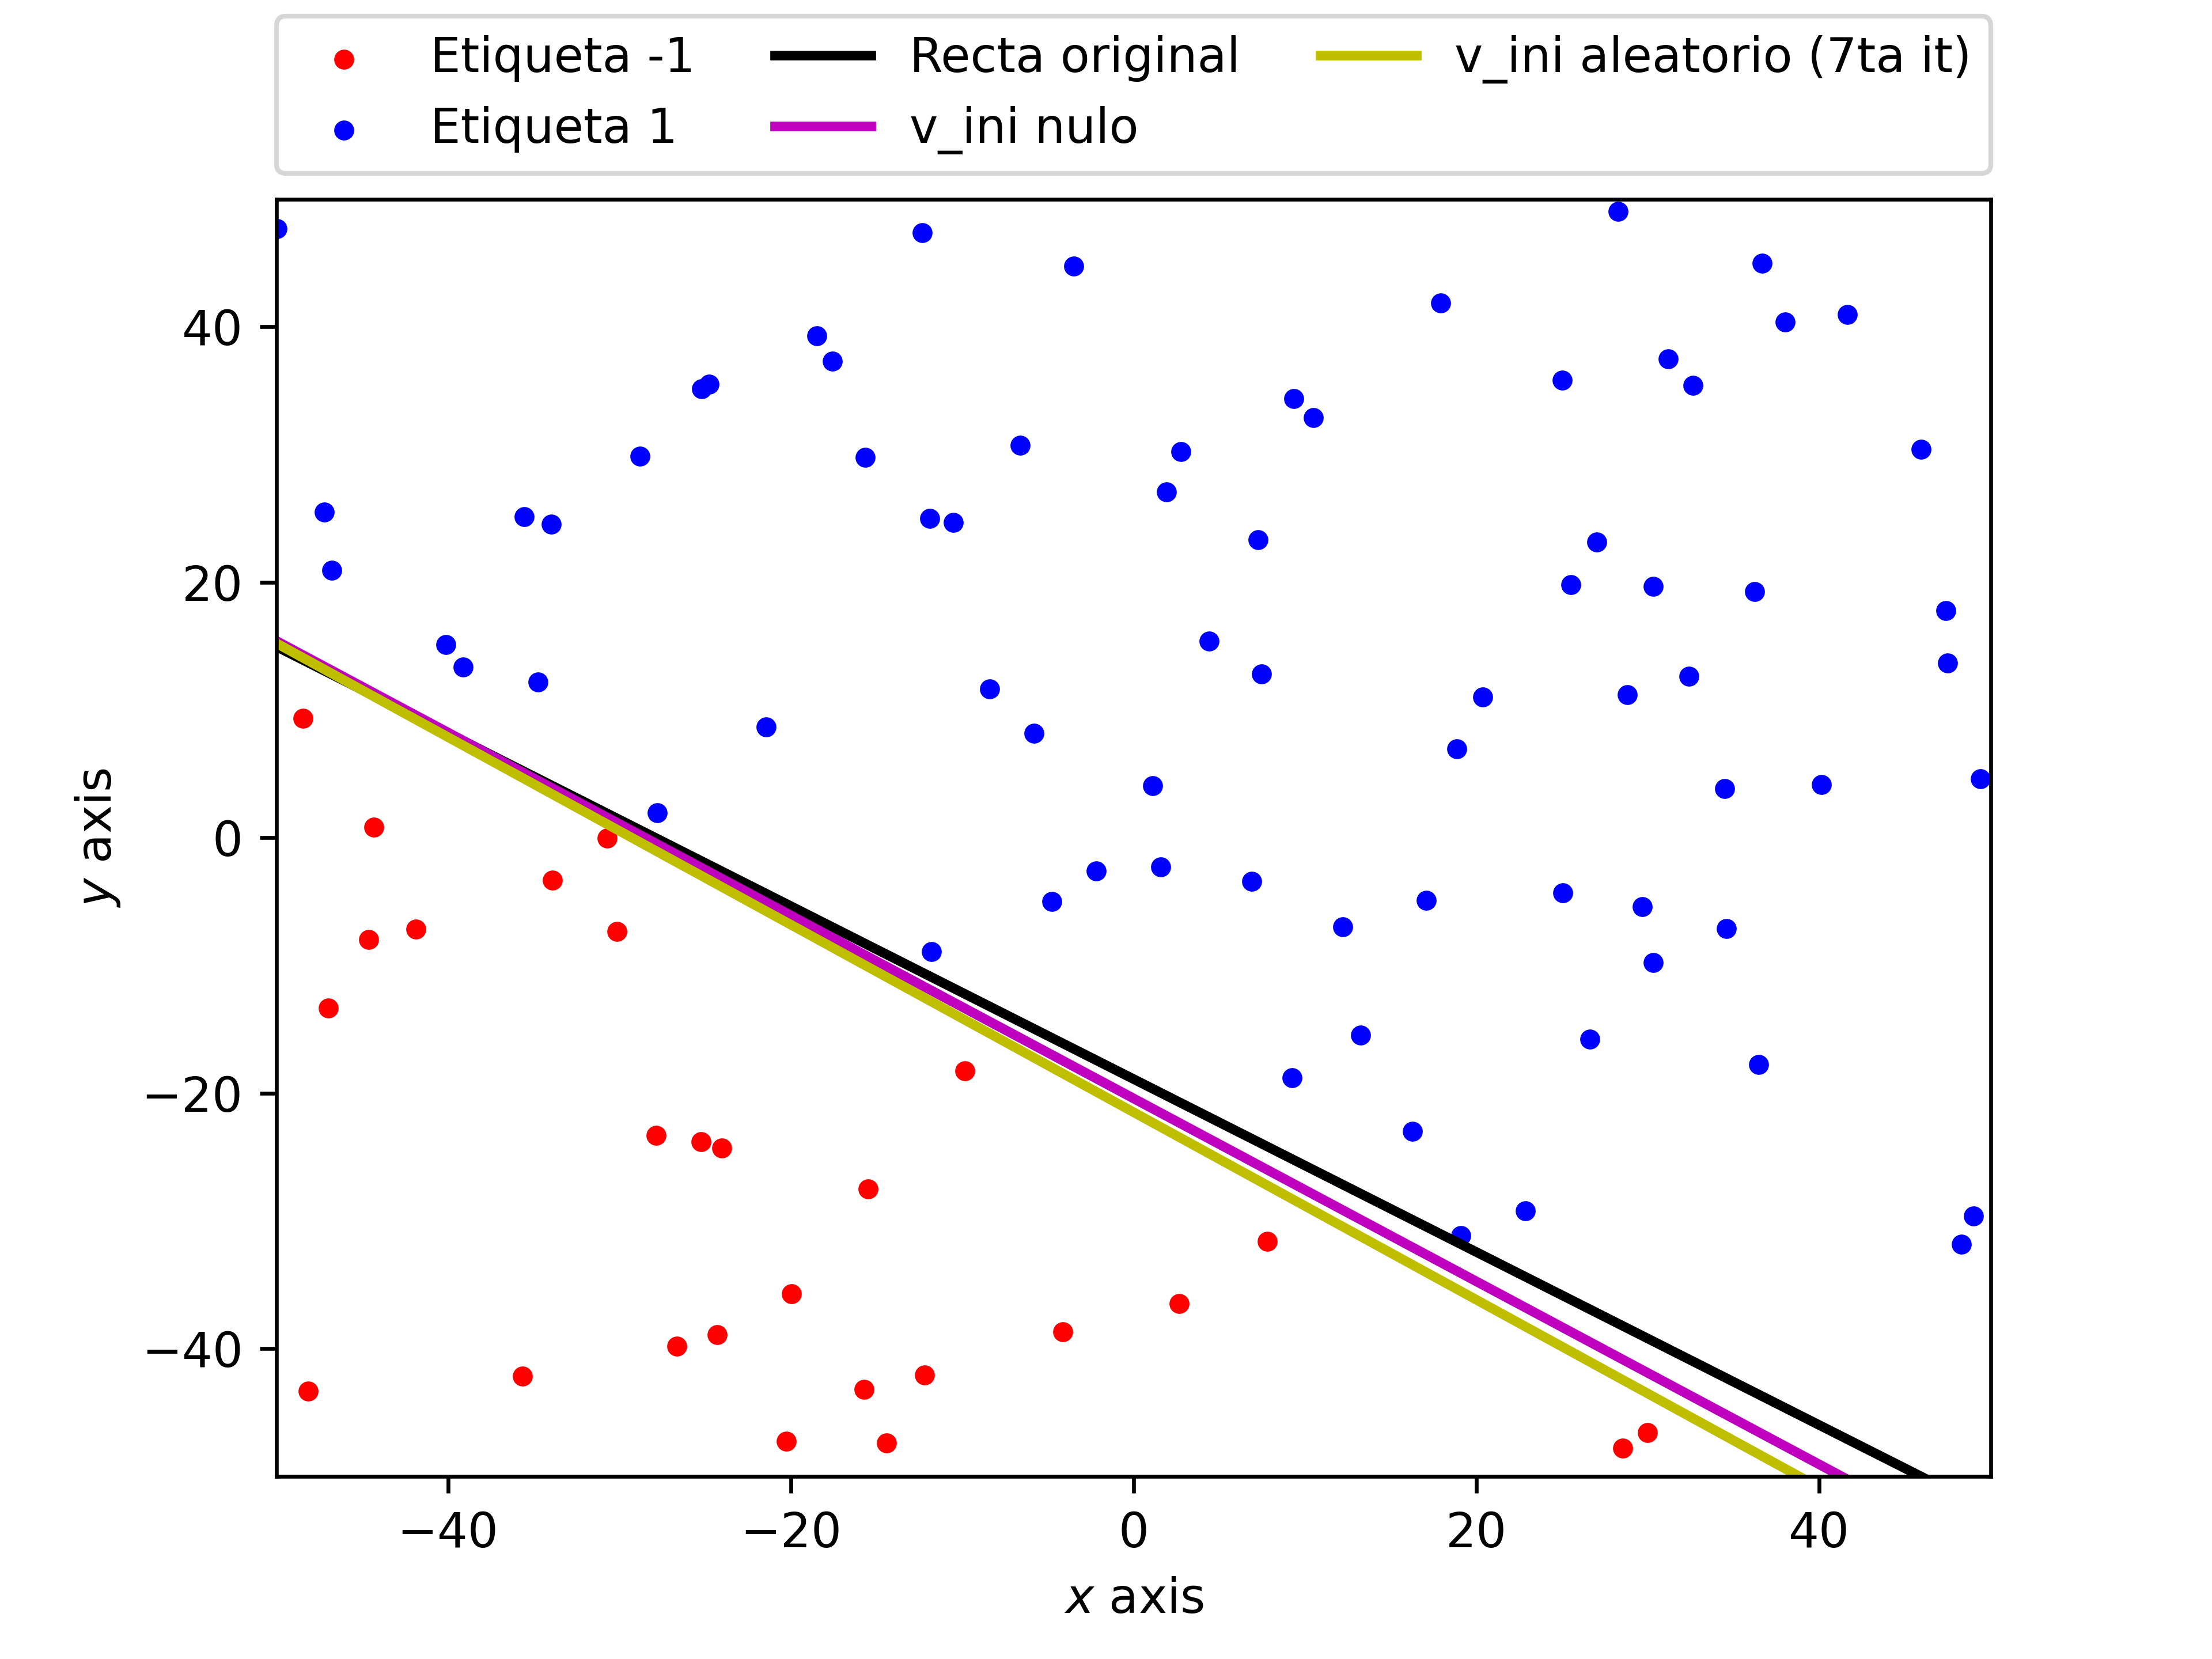
\includegraphics[scale=0.6]{Figure_10.png}
\caption{Regresión con características no lineales $\Phi(x)$}
\end{figure}

\section{Comparación entre los experimentos}

A la vista de los resultados de los errores promedios $E_{in}$ y $E_{out}$
obtenidos en los dos experimentos, \textbf{¿qué modelo considera que es el más
adecuado? Justifique la respuesta.}

\hfill \break

La figura generada encaja con los resultados. El modelo con características no
lineales aplica una transformación donde la regresión lineal calculada con el
algoritmo de gradiente descendente estocástico con $200$ iteraciones y $\eta=0.01$
arroja unos errores de ajustes menores ($E_{in} \approx 0.7738$ , $E_{out} \approx = 0.778$),
que sin la transformacíón ($E_{in} \approx 0.9320$, $E_{out} \approx 0.9357$).